\documentclass[a4paper,12pt]{article}
%\usepackage[T2A]{fontenc}
\usepackage[utf8]{inputenc}
%\usepackage[english]{babel}
\usepackage{amsmath}
\usepackage{amsfonts}
\usepackage{amssymb}
\usepackage{multicol}
\usepackage{geometry}
\usepackage[pdftex]{graphicx}
\usepackage{hyperref}
\usepackage{indentfirst}
\hypersetup{colorlinks=true}
%\renewcommand{\baselinestretch}{1.5}
%\usepackage[left=2cm,right=2cm,top=2cm,bottom=2cm]{geometry}
\geometry{hmargin={20mm,20mm},vmargin={20mm,20mm}}
%opening
\setcounter{tocdepth}{3} 

\begin{document}
\large
%\maketitle
\begin{titlepage}
 \begin{center}
Warsaw University of Technology\\
The Faculty of Electronics and Information Technology
  
  \vspace{35ex}
  
Contemporary Heuristic Techniques  course project\\
subject:\\
''Application of the Artificial neural networks in the approximation task''

  
  \vspace{35ex}
  
 \end{center}
 \begin{flushright}
Supervisor:\\
Piotr Bilski\\
Made by:\\
Oleksandr Halushko\\
Danylo Lizanets

\vspace{15ex}

 \end{flushright}
  
  \begin{center}
   Warsaw 2013
  \end{center}

\end{titlepage}

\tableofcontents
\newpage
\section{Subject}

Application of the artificial neural networks in the approximation task.

\section{Aim}

Apply the artificial neural network to approximate a two-dimensional function. Design the structure of the network and make it learn the selected number of the points being a part of the function, then test it against the new set of the points. Test different structures of the network. Examine the learning process of the designed network.

\section{Advanced theory}
\subsection{Artificial neural networks}
\subsubsection{Definition}

Artificial neural network is a mathematical model of biological neural network. It consists of artificial neurons and processes information using a connectionist approach to computation. Neural networks are used for modeling complex relationships between inputs and outputs or searching of patterns in data.

\subsubsection{Types of artificial neural networks}

There are many different types of the artificial neural networks used for different purposes. They may be classified by such parameters as:
\begin{itemize}
 \item number of layers
  \begin{itemize}
   \item one layer
   \item two layers
   \item multilayer
  \end{itemize}
  \item number of information move directions
  \begin{itemize}
   \item one direction
   \item many directions
  \end{itemize}
  \item number of inputs
  \begin{itemize}
   \item single input 
   \item multiple input
  \end{itemize}
  \item existance of recursive feedback loops
  \item type of learning
  \begin{itemize}
   \item outside teaching
   \item self-teaching
  \end{itemize}

\end{itemize}


 %(one-, two-, multilayer),  directions(one, many), inputs (single, multiple), existance of recursive feedback loops and type of learning. 

The feed-forward neural network is the most simple type of artificial neural network. In this type network the information moves in only one direction — forwards: from the input nodes data goes through the hidden nodes and to the output nodes. There are no cycles or loops in the network.

\subsubsection{Activation functions and their influences on the training process}

In computational networks, the activation function of a node defines the output of that node given an input or set of inputs.

In biologically inspired neural networks, the activation function is usually an abstraction representing the rate of action potential firing in the cell. In its simplest form, this function is binary—that is, either the neuron is firing or not. The function looks like $\phi(v_i)=U(v_i)$ , where $U$ is the Heaviside step function. In this case a large number of neurons must be used in computation beyond linear separation of categories.

A line of positive slope may also be used to reflect the increase in firing rate that occurs as input current increases. The function would then be of the form $\phi(v_i)=\mu v_i$, where $\mu$ is the slope. This activation function is linear, and therefore has the same problems as the binary function. In addition, networks constructed using this model have unstable convergence because neuron inputs along favored paths tend to increase without bound, as this function is not normalizable.

All problems mentioned above can be handled by using a normalizable sigmoid activation function. One realistic model stays at zero until input current is received, at which point the firing frequency increases quickly at first, but gradually approaches an asymptote at 100\% firing rate. Mathematically, this looks like $\phi(v_i)=U(v_i)\tanh(v_i)$, where the hyperbolic tangent function can also be any sigmoid. This behavior is realistically reflected in the neuron, as neurons cannot physically fire faster than a certain rate. This model runs into problems, however, in computational networks as it is not differentiable, a requirement in order to calculate backpropagation.

The final model, then, that is used in multilayer perceptrons is a sigmoidal activation function in the form of a hyperbolic tangent. Two forms of this function are commonly used: $\phi(v_i)=\tanh(v_i)$ whose range is normalized from -1 to 1, and $\phi(v_i) = (1+\exp(-v_i))^{-1}$ is vertically translated to normalize from 0 to 1. The latter model is often considered more biologically realistic, but it runs into theoretical and experimental difficulties with certain types of computational problems.

Linear discriminant functions, as the name suggests, can differentiate between two classes of data that are bounded by a hyperplane. In two dimensions, a hyperplane is just a line, and in three dimensions it is a standard plane. These functions are often convenient for separating classes of data from different distributions\cite{nn}.

A sigmoid function $1/(1 + e^{-\beta} )$ is often used as an activation function for neurons in a neural network. When the activation is strongly positive, the neuron responds with values close to 1.0. When the activation is strongly negative, the neuron responds with values close to 0.0. For activations in the range of $[-1 ,1]$ the sigmoid function is close to linear, but then saturates in both directions.\cite{nn}

\subsubsection{Training process}

Training a neural network model essentially means selecting one model from the set of allowed models that minimizes the cost criterion.

A commonly used cost is the mean-squared error, which tries to minimize the average squared error between the network's output, $f(x)$, and the target value y over all the example pairs. When one tries to minimize this cost using gradient descent for the class of neural networks called multilayer perceptrons, one obtains the common and well-known backpropagation algorithm for training neural networks.

There are three major learning paradigms, each corresponding to a particular abstract learning task. These are supervised learning, unsupervised learning and reinforcement learning.

In \emph{supervised learning}, we are given a set of example pairs $ (x, y), x \in X, y \in Y $ and the aim is to find a function $ f : X \rightarrow Y $ in the allowed class of functions that matches the examples. In other words, we wish to infer the mapping implied by the data; the cost function is related to the mismatch between our mapping and the data and it implicitly contains prior knowledge about the problem domain.

A commonly used cost is the mean-squared error, which tries to minimize the average squared error between the network's output, $f(x)$, and the target value y over all the example pairs. When one tries to minimize this cost using gradient descent for the class of neural networks called multilayer perceptrons, one obtains the common and well-known backpropagation algorithm for training neural networks.

Tasks that fall within the paradigm of supervised learning are pattern recognition (also known as classification) and regression (also known as function approximation). The supervised learning paradigm is also applicable to sequential data (e.g., for speech and gesture recognition). This can be thought of as learning with a "teacher," in the form of a function that provides continuous feedback on the quality of solutions obtained thus far.

In \emph{unsupervised learning}, some data $ x $ is given and the cost function to be minimized, that can be any function of the data $ x $ and the network's output, $f$

The cost function is dependent on the task (what we are trying to model) and our a priori assumptions (the implicit properties of our model, its parameters and the observed variables).

As a trivial example, consider the model $f(x) = a$, where $ a $ is a constant and the cost $ C=E[(x - f(x))^2] $. Minimizing this cost will give us a value of $ a $ that is equal to the mean of the data. The cost function can be much more complicated. Its form depends on the application: for example, in compression it could be related to the mutual information between $ x $ and $ f(x) $, whereas in statistical modeling, it could be related to the posterior probability of the model given the data. (Note that in both of those examples those quantities would be maximized rather than minimized).

Tasks that fall within the paradigm of unsupervised learning are in general estimation problems; the applications include clustering, the estimation of statistical distributions, compression and filtering.

In \emph{reinforcement learning}, data $ x $ are usually not given, but generated by an agent's interactions with the environment. At each point in time $ t $, the agent performs an action $ y_t  $ and the environment generates an observation $ x_t $ and an instantaneous cost $ c_t $, according to some (usually unknown) dynamics. The aim is to discover a policy for selecting actions that minimizes some measure of a long-term cost; i.e., the expected cumulative cost. The environment's dynamics and the long-term cost for each policy are usually unknown, but can be estimated.

More formally, the environment is modeled as a Markov decision process (MDP) with states $ \{s_1,...,s_n\}\in S $ and actions $\{a_1,...,a_m\} \in A $ with the following probability distributions: the instantaneous cost distribution $ P(c_t|s_t) $, the observation distribution $ P(x_t|s_t) $ and the transition $ P(s_{t+1}|s_t, a_t), $ while a policy is defined as conditional distribution over actions given the observations. Taken together, the two define a Markov chain (MC). The aim is to discover the policy that minimizes the cost; i.e., the MC for which the cost is minimal.

Tasks that fall within the paradigm of reinforcement learning are control problems, games and other sequential decision making tasks.

\subsection{Approximation}
\subsubsection{What approximation is}

Function approximation, which finds the underlying relationship from a given finite input-output data is the fundamental problem in a vast majority of real world applications, such as prediction, pattern recognition, data mining and classification. Various methods have been developed to address this problem, where one of them is by using artificial neural networks.

\subsubsection{Artificial neural network using for function approximation}

Due to the universal approximation theorem, the standard multilayer feed-forward neural network with a single hidden layer, which contains finite number of hidden neurons, is a universal approximator for continuous functions on compact subsets of $R^n$.

Let $\varphi(\bullet) $ be a non constant, bounded, and monotonically-increasing continuous function. Let $I_m$ denote the m-dimensional unit hypercube $ [0,1]_m. $ The space of continuous functions on $ I_m $ is denoted by $C(I_m)$. Then, given any function $ f \in C(I_m) $ and $ \varepsilon > 0 $, there exist an integer $ N $ and real constants $ \alpha_i, b_i \in R, \omega_i \in Rm $, where $ i = 1, \hdots, N $ such that we may define:

\begin{equation}
 F(x) = \sum\limits_{i=1}^N\alpha_i\varphi(\omega_i^Tx+b_i) 
\end{equation}

as an approximate realization of the function $ f $ ; that is,

\begin{equation}
 |F(x)-f(x)|<\varepsilon
\end{equation}

for all $ x \in I_m$. In other words, function of the form $ F(x) $ are dence in $ C(I_m) $.   
\begin{figure}[ht]
 \centering
 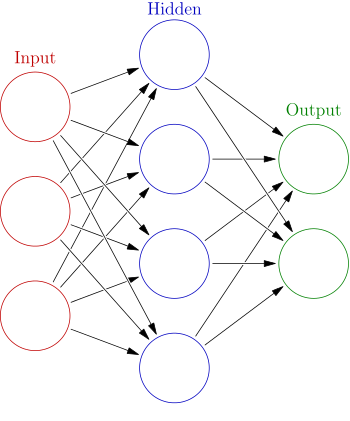
\includegraphics[scale=0.4]{images/neurons.png}
 \caption{Neural network with one hidden layer}
\end{figure}

\subsection{Backpropagation}

Backpropagation, an abbreviation for "backward propagation of errors", is a common method of training artificial neural networks. From a desired output, the network learns from many inputs, similar to the way a child learns to identify a dog from examples of dogs.

It is a supervised learning method, and is a generalization of the delta rule. It requires a data set of the desired output for many inputs, making up the training set. It is most useful for feed-forward networks (networks that have no feedback, or simply, that have no connections that loop). Backpropagation requires that the activation function used by the artificial neurons (or "nodes") be differentiable.

There are three modes of learning to choose from: on-line, batch and stochastic. In on-line and stochastic learning, each propagation is followed immediately by a weight update. In batch learning, many propagation occur before updating the weights. Batch learning requires more memory capacity, but on-line and stochastic learning require more updates. On-line learning is used for dynamic environments that provide a continuous stream of new patterns. Stochastic learning and batch learning both make use of a training set of static patterns. Stochastic goes through the data set in a random order in order to reduce its chances of getting stuck in local minimum. Stochastic learning is also much faster than batch learning since weights are updated immediately after each propagation. Yet batch learning will yield a much more stable descent to a local minimum since each update is performed based on all patterns.

\subsubsection{Propagation}
\begin{itemize}

 \item \emph{Phase 1}: Propagation

Each propagation involves the following steps:
\begin{enumerate}
 \item Forward propagation of a training pattern's input through the neural network in order to generate the propagation's output activations.
 \item Backward propagation of the propagation's output activations through the neural network using the training pattern target in order to generate the deltas of all output and hidden neurons.
\end{enumerate}

\item \emph{Phase 2}: Weight update

For each weight-synapse follow the following steps:
\begin{enumerate}
 \item Multiply its output delta and input activation to get the gradient of the weight.
 \item Bring the weight in the opposite direction of the gradient by subtracting a ratio of it from the weight.
\end{enumerate}

This ratio influences the speed and quality of learning; it is called the learning rate. The sign of the gradient of a weight indicates where the error is increasing, this is why the weight must be updated in the opposite direction.

Repeat phase 1 and 2 until the performance of the network is satisfactory.
\end{itemize}

\subsubsection{Limitations}

\begin{itemize}

 \item The result may converge to a local minimum. The "hill climbing" strategy of gradient descent is guaranteed to work if there is only one minimum. However, oftentimes the error surface has many local minimum and maximum. If the starting point of the gradient descent happens to be somewhere between a local maximum and local minimum, then going down the direction with the most negative gradient will lead to the local minimum.
    \item Gradient descent can find the local minimum instead of the global minimum
    \item The convergence obtained from backpropagation learning is very slow.
    \item The convergence in backpropagation learning is not guaranteed.
    \item Backpropagation learning does not require or normalization of input vectors; however, normalization could improve performance.[8]
\end{itemize}

\subsubsection{Network error function and precision measures}

Since backpropagation uses the gradient descent method, one needs to calculate the derivative of the squared error function with respect to the weights of the network. The squared error function is (the $\frac{1}{2}$ term is added to cancel the exponent when differentiating):

\begin{equation}
 E = \frac{1}{2}(t-y)^2,
\end{equation}
 $E = \text{squared error}$\\ 
 $t = \text{target output}$\\ 
 $y = \text{actual output of the output neuron}$\\


 Therefore the error, $E$, depends on the output $y$ . However, the output y depends on the weighted sum of all its input:
\begin{equation}
  	y = \sum_{i=1}^{n}w_ix_i
\end{equation}
	$n = \text{the number of input units to the neuron}$\\
	$w_i = \text{the ith weight}$\\
	$x_i = \text{the ith input value to the neuron}$\\


The above formula only holds true for a neuron with a linear activation function (that is the output is solely the weighted sum of the input). In general, a non-linear, differentiable activation function, $\varphi$, is used. Thus, more correctly:
\begin{equation}
 	y = \varphi(net), 
	net = \sum_{i=1}^{n}w_ix_i
\end{equation}

This lays the groundwork for calculating the partial derivative of the error with respect to a weight $w_i$ using the chain rule:
\begin{equation}
 	\frac{\partial E}{\partial w_i} = \frac{dE}{dy} \frac{dy}{dnet} \frac{\partial net}{\partial w_i}
\end{equation}
	$\frac{\partial E}{\partial w_i} = \text{How the error changes when the weights are changed}$\\
	$\frac{dE}{dy} = \text{How the error changes when the output is changed}$\\
	$\frac{dy}{dnet} = \text{How the output changes when the weighted sum changes}$\\
	$\frac{\partial net}{\partial w_i} = \text{How the weighted sum changes as the weights change}$\\

Since the weighted sum net is just the sum over all products $w_i x_i$, therefore the partial derivative of the sum with respect to a weight $w_i$ is the just the corresponding input $x_i$. Similarly, the partial derivative of the sum with respect to an input value $x_i$ is just the weight $w_i$:
\begin{equation}
 	\frac{\partial net}{\partial w_i} = x_i
\end{equation}
\begin{equation}
	\frac{\partial net}{\partial x_i} = w_i
\end{equation}

The derivative of the output y with respect to the weighted sum net is simply the derivative of the activation function $\varphi$:
\begin{equation}
     \frac{dy}{dnet} = \frac{d}{dnet}\varphi 
\end{equation}
This is the reason why backpropagation requires the activation function to be differentiable. A commonly used activation function is the logistic function:
\begin{equation}
    y = \frac{1}{1+e^{-z}}
\end{equation}

which has a nice derivative of:
\begin{equation}
     \frac {dy}{dt} = y(1-y) 
\end{equation}

For example purposes, assume the network uses a logistic activation function, in which case the derivative of the output y with respect to the weighted sum net is the same as the derivative of the logistic function:
\begin{equation}
     \frac {dy}{dnet} = y(1-y) 
\end{equation}

Finally, the derivative of the error E with respect to the output y is:
\begin{equation}
 	\frac{dE}{dy} = \frac {d}{dy} \frac{1}{2}(t - y)^2
\end{equation}
\begin{equation}
	\frac{dE}{dy} = y - t
\end{equation}

Putting it all together:
\begin{equation}
 	\frac{\partial E}{\partial w_i} = \frac{dE}{dy} \frac{dy}{dnet} \frac{\partial net}{\partial w_i}
	\frac{\partial E}{\partial w_i} = (y - t) y (1 - y) x_i
\end{equation}

If one were to use a different activation function, the only difference would be the y $(1 - y)$ term will be replaced by the derivative of the newly chosen activation function.

To update the weight $w_i$ using gradient descent, one must chooses a learning rate, $\alpha$. The change in weight after learning then would be the product of the learning rate and the gradient:
\begin{equation}
 	\Delta w_i = - \alpha \frac{\partial E}{\partial w_i}
	\Delta w_i = \alpha (t - y) \varphi' x_i
\end{equation}

For a linear neuron, the derivative of the activation function $\varphi$ is 1, which yields:
\begin{equation}
     \Delta w_i = \alpha (t - y) x_i 
\end{equation}

This is exactly the delta rule for perceptron learning, which is why the backpropagation algorithm is a generalization of the delta rule. In backpropagation and perceptron learning, when the output y matches the desired output t, the change in weight $\Delta w_i$ would be zero, which is exactly what is desired.

 
\section{Domain description}

\subsection{Function}
Function for approximation we are using in our project is ''Sombrero'' function which formula is such:
\begin{equation}
 t = \sqrt{((a+bx)^2+(a+by)^2)} \text{, where } a = -8, b = 16
 \end{equation}
 \begin{equation}
 z = \frac
 {\sin(t)}
 {t}
\end{equation}

The function is mapped on $[0,1]_2$ hypercube due to the requirements of universal approximation theorem.

\section{Application description}

\subsection{Application structure}

For testing and training neural networks was developed GUI application, which allows user to create neural networks, set different parameters of it and give it data sets for training and  testing to obtain appropriate results. The application consists of three parts: Neural Network, IO/Preparing data, GUI. 

\subsubsection{Classes}
\begin{itemize}
 \item Facade - connects all parts of the application together, receiving information and commands from other classes, and sends them to recipient;
 \begin{figure}[!ht]
 \centering
 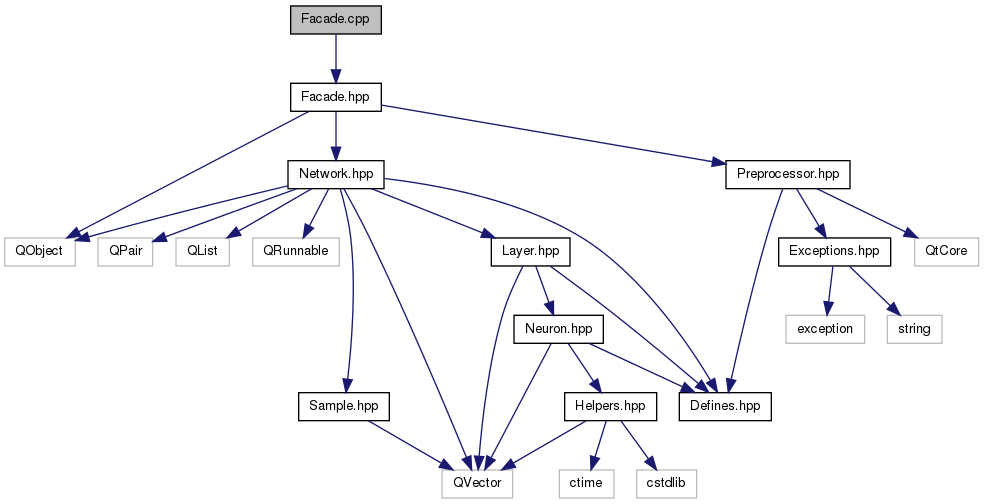
\includegraphics[scale=0.4]{images/facadecppincl.png}
 \caption{Facade class connections}
\end{figure}

 \begin{figure}[!ht]
 \centering
 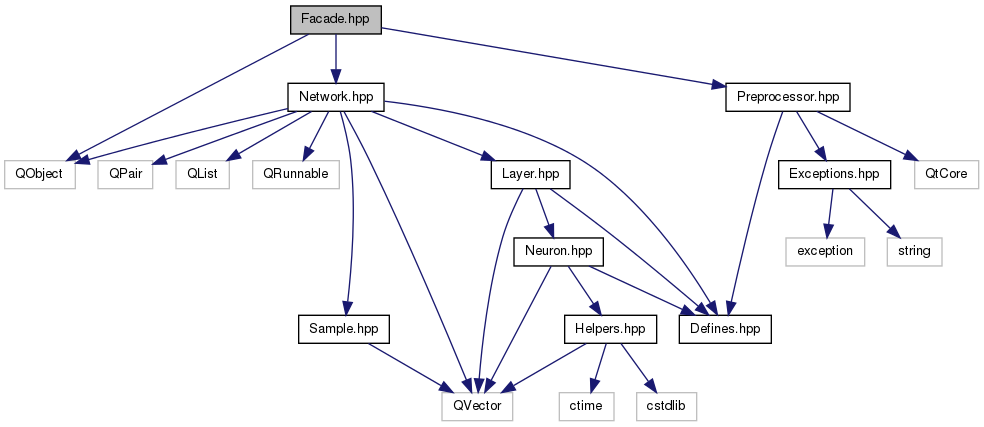
\includegraphics[scale=0.4]{images/facadehppincl.png}
 \caption{Facade class connections}
\end{figure}

\item Network - represents artificial neural network, gets parameters of network and training/testing data samples, returns results for testing data and array of error values for epochs.
Activation functions is stored in separate file Helpers.hpp, that gives ability to change them easily for creating different types of neural networks.

 \begin{figure}[!ht]
 \centering
 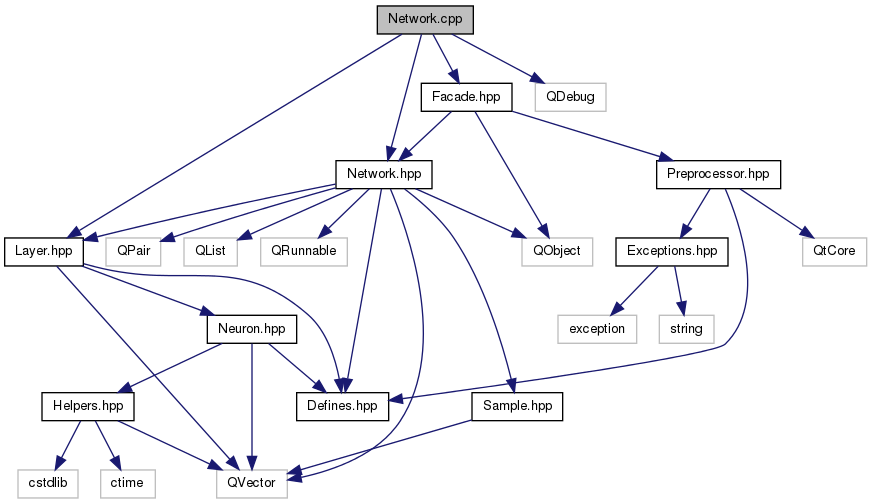
\includegraphics[scale=0.4]{images/networkcppincl.png}
 \caption{Network class connections}
\end{figure}

 \begin{figure}[!ht]
 \centering
 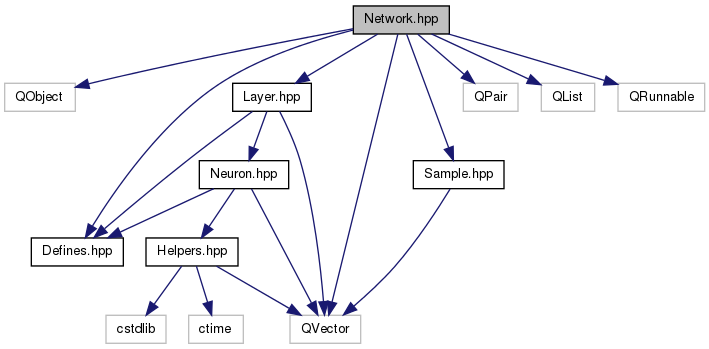
\includegraphics[scale=0.4]{images/networkhppincl.png}
 \caption{Network class connections}
\end{figure}

\item Layer - represents an one layer of artificial neural network, gets parameters that define number of neurons in layer and number of inputs of single neuron.

\item Neuron - represents a single neuron of artificial neural network.

\item Preprocessor - reads and writes data to files, prepares data for further transmission to artificial neural network by splitting it to training and testing sets of input and output parameters.

 \begin{figure}[!ht]
 \centering
 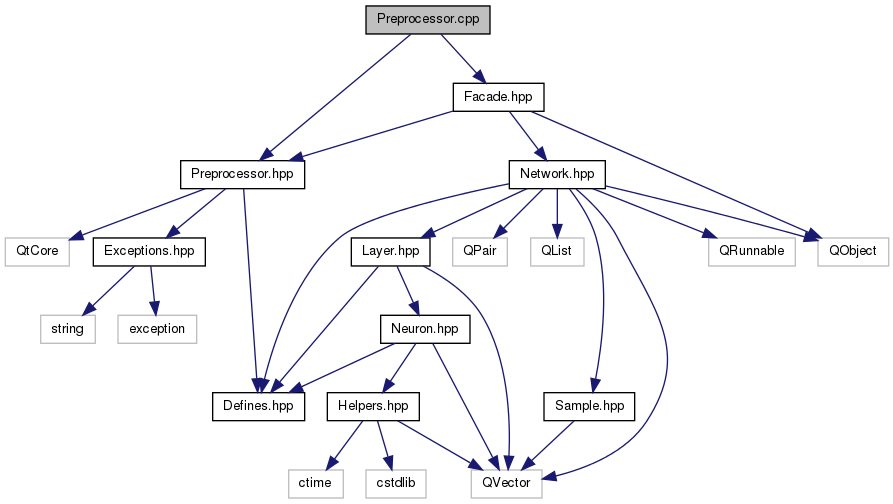
\includegraphics[scale=0.4]{images/preprocessorcppincl.png}
 \caption{Preprocessor class connections}
\end{figure}

\item MainWindow - represents GUI of application, contains controls for setting parameters of artificial neural networks.

\end{itemize}

\subsection{Application interface}

Graphical user interface of application consists of 5 parts: DataSource, Control, Layer Settings, Results, Graph of errors.

In DataSource user can open file with data samples for artificial neural network. Based on this file application will automatically set the number of neurons and inputs in each neuron in one hidden layer of artificial neural network. 

Control allow user to set such parameters of artificial neural network as training coefficient, stretching coefficient, precision, maximum number of epoch and percent of testing data. 

In Layer Settings can be set number of layers of artificial neural network, number of neurons for each layer and number of inputs for neurons in each layer. 

In Results are displayed results of testing the artificial neural network with ability to store it to file. 

Graph of errors shows error dependency from number of epoch.

\begin{figure}[!h]
 \centering
 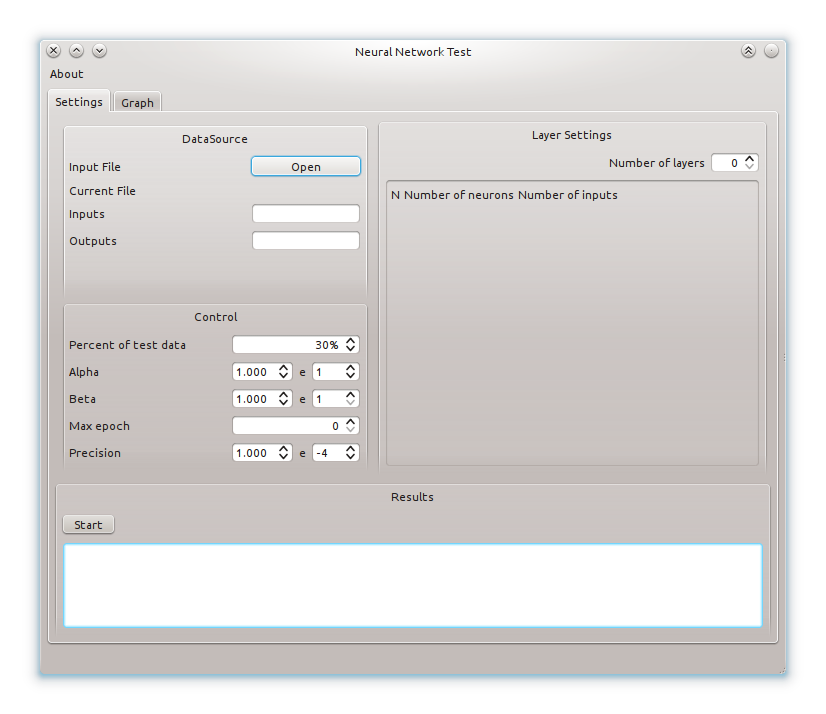
\includegraphics[scale=0.5]{images/interface.png}
 \caption{Application interface}
\end{figure}

\begin{figure}[!h]
 \centering
 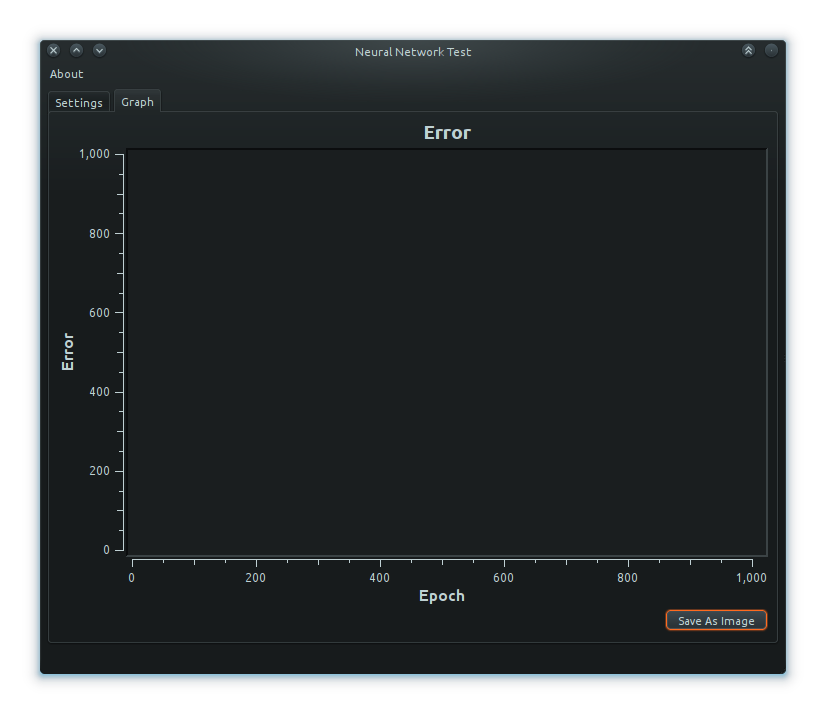
\includegraphics[scale=0.5]{images/interface1.png}
 \caption{Graphical error representation}
\end{figure}

\newpage
\newpage

\begin{thebibliography}{9}

\bibitem{nn}
  Zbigniew Michalewicz, David B. Fogel
  \emph{How to Solve It: Modern Heuristics}.
  Springer,
  2nd Edition,
  2000
\bibitem{wiki}
  \emph{wikipedia.org}
\end{thebibliography}

\end{document}




